% !TEX root = ../main.tex
\subsection{Trajektóriák és mozgásleírás CDR-ből}
A CDR adatok időrendbe rendezett cellasorozatokként értelmezhetők. Egy előfizető
útvonala $T_{a}=\{(c_{1},t_{1}),(c_{2},t_{2}),\dots,(c_{n},t_{n})\}$, ahol
$c_{i}$ a kiszolgáló cella azonosítója, $t_{i}$ pedig az esemény időpontja. A
cella koordinátái vagy a torony centruma külön adattáblából származnak. A rekonstrukció
során jellemzően \textbf{időintervallum-alapú interpolációt} alkalmaznak. Az események
közötti időszakot ilyenkor a felhasználó \textbf{utolsó ismert cellájához}
rendelik. Emellett számolnak azzal is, hogy a cellaváltások egy része pusztán
\textbf{handover folyamat}, és nem feltétlenül valódi helyváltoztatás
\cite{pinter2022awakening}.

\subsection{Radius of Gyration (gyrációs sugár)}

A gyrációs sugár ($r_{g}$) az egyéni mobilitás hatótávolságának alapvető mérőszáma,
amely a meglátogatott helyek tömegközépponttól való átlagos négyzetes távolságát
fejezi ki \cite{pinter2021evaluating}. Jelölje $N$ a vizsgált időszakban rögzített
események számát, $\vec{r}_{i}$ az $i$-edik esemény helyszínének koordinátáit, $\vec
{r}_{\mathrm{cm}}= \frac{1}{N}\sum_{i=1}^{N}\vec{r}_{i}$ pedig a trajektória tömegközéppontját.
Ekkor a gyrációs sugár definíciója:

\begin{equation}
	r_{g} = \sqrt{\frac{1}{N}\sum_{i=1}^{N}\|\vec{r}_{i} - \vec{r}_{\mathrm{cm}}\|^{2}}
	.
\end{equation}
\begin{figure}[h!]
    \centering
    % A képfájl neve:
    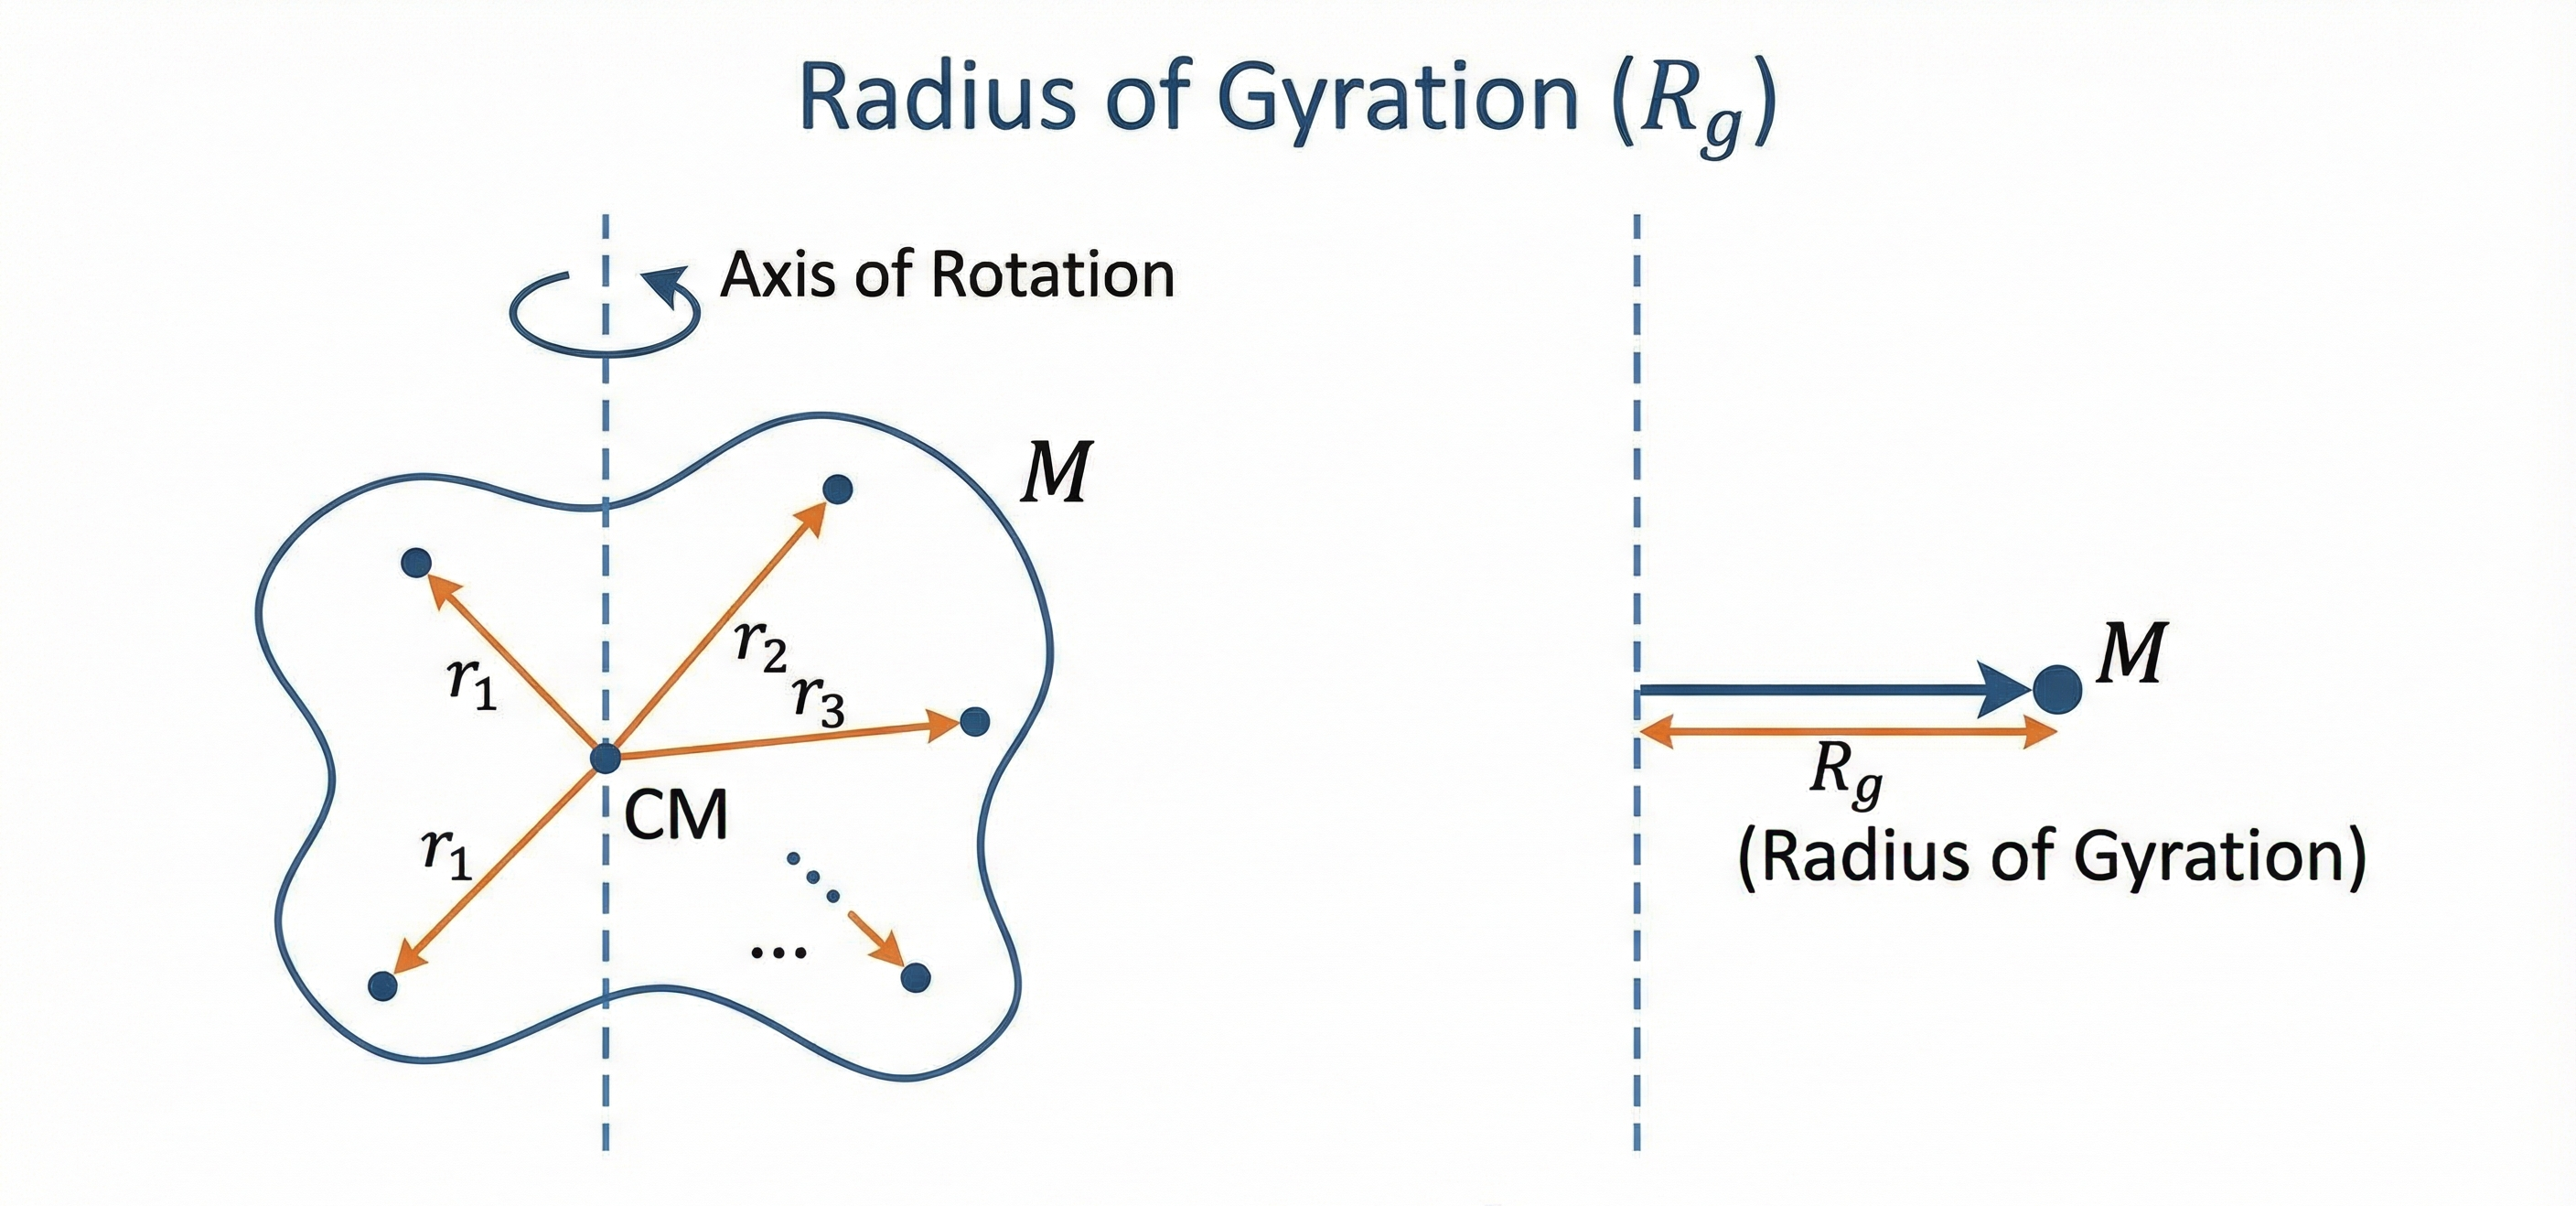
\includegraphics[width=0.6\textwidth]{img/radius_of_gyration.png}
    
    % Rövid cím (ábrajegyzékbe):
    \caption[A gyrációs sugár (Radius of Gyration) szemléltetése]{A gyrációs sugár ($r_g$) szemléltetése. \\ \footnotesize\textit{Forrás: AI generált kép}}
    
    % Hivatkozási címke:
    \label{fig:radius_gyration}
\end{figure}


A metrika eloszlása a populációban egy vágott hatványfüggvénnyel (truncated
power-law) közelíthető:
$P(r_{g}) \sim (r_{g}+r_{0})^{-\beta_r}\exp(-r_{g}/\kappa)$. González és munkatársai \cite{gonzalez2008understanding}
mérései alapján a jellemző paraméterek $r_{0} \approx 5{,}8$ km, $\beta_{r}\approx
1{,}65$ és a vágási érték $\kappa \approx 350$ km. A kutatások kimutatták, hogy az
$r_{g}$ időbeli növekedése csupán logaritmikus ütemű, ami arra utal, hogy az emberi
mozgás nem véletlenszerű diffúzió, hanem térben korlátozott és erősen visszatérő
jellegű \cite{gonzalez2008understanding}.






\subsection{Egyéb gyakori mobilitási metrikák}
\begin{itemize}
	\item \textbf{Látogatott egyedi helyek száma.} Egy adott időszakban
		meglátogatott különböző cellák számát $S$ jelöli. Nagy $S$ érték tág mozgási
		repertoárt jelez, míg kis $S$ koncentrált mozgást.

	\item \textbf{Napi/heti megtett távolság.} Az egymást követő cellák közötti
		távolságok összege. A metrika alulbecsülheti a tényleges útvonalat a pontos hely
		ismerete hiányában \cite{gonzalez2008understanding}.

	\item \textbf{Entrópia alapú mutatók.} A térbeli entrópia
		$H_{s} = -\sum_{j} p_{j} \log p_{j}$ a felhasználó cellalátogatási
		eloszlásából számítható, ahol $p_{j}$ a $j$-edik cella látogatási
		valószínűsége \cite{pinter2021evaluating}. A magas entrópia változatos térhasználatra,
		míg az alacsony érték kevés helyre koncentrálódó, kiszámítható mozgásra utal.
		\cite{pinter2022awakening}.

	\item \textbf{Home és work cella detektálása.} A leggyakoribb éjszakai hely az
		otthon, a Leggyakoribb nappali pedig a munkahely\cite{pinter2021evaluating, pinter2022awakening}

\end{itemize}

\subsection{Kiegészítő napi metrikák}
\label{subsec:extra_metrics}

A gyrációs sugár, az entrópia és a helydiverzitás mellett a CDR-szakirodalomban gyakran használt további napi metrikák, amelyeket a megvalósított rendszer (7.\ fejezet) szintén kiszámít:

\begin{itemize}
	\item \textbf{Aktivitáskoncentráció (AC).} A felhasználó napi pingjeinek hányadrésze esik a top~$k$ leglátogatottabb cellára:
		\[
		\mathrm{AC}_k = \frac{\sum_{j \in \mathrm{top}_k} n_j}{\sum_j n_j}, \qquad k = 3.
		\]
		Magas $\mathrm{AC}$ erősen koncentrált térhasználatot jelez. A korlátozó intézkedések (lockdown, vészhelyzet) tipikusan növelik az értékét \cite{pinter2022awakening}.

	\item \textbf{Visszatérési ráta (RR).} Az adott napon érintett cellák hányadrésze, amelyek az előző napon is érintettek voltak:
		\[
		\mathrm{RR}(d) = \frac{|C_d \cap C_{d-1}|}{|C_d|}, \qquad C_d = \{(x,y) \text{ cellák a } d \text{ napon}\}.
		\]
		Magas $\mathrm{RR}$ erős napi rutint, kiszámítható mozgást jelent. A González-féle visszatérő mozgásmodellel \cite{gonzalez2008understanding} áll rokonságban.

	\item \textbf{Csúcsidőrés (peak slot).} Az a 30~perces időrés ($t \in \{0,\dots,47\}$), amelyikben a felhasználó napi pingszáma maximális. A reggeli/esti ingázási csúcs \cite{pinter2022awakening} egyéni szintű proxyja.

	\item \textbf{Hétvége-jelző (weekend flag).} Bináris jelölő: $d \bmod 7 \in \{0, 6\}$ esetén hétvége. A hét napjainak sorrendjét empirikusan kell megállapítani, mert a YJMob100K nem hozza nyilvánosságra a kezdő dátumot (a levezetést a 9.\ fejezet validálja).
\end{itemize}